\documentclass{article}
\usepackage[utf8]{inputenc}

\title{CS 376 Hybrid Systems}
\author{Fred Eisele}
\date{November 2014}

\usepackage{graphicx}
\usepackage{tikz}
\usetikzlibrary{shapes,arrows}
\usepackage{amsmath}
\usepackage{amsfonts}
\usepackage{xfrac}

\begin{document}

\maketitle

\tikzstyle{block} = [draw, fill=blue!20, rectangle,
    minimum height=3em, minimum width=6em]


\section{Hybrid Timed Automaton}
Construct a timed automaton that produces $tick$
events in a periodic pattern.

\begin{equation}
1, 2, 3, 5, 6, 7 ,8, 10, 11, \ldots
\end{equation}

\ldots or the times between events \ldots

\begin{equation}
1, 1, 1, 2, 1, 1, 1, 2, 1, 1, \ldots
\end{equation}

That is three $tick$ events one second apart
and one $tick$ event two seconds later repeated.

\begin{figure}[h!]
\centering
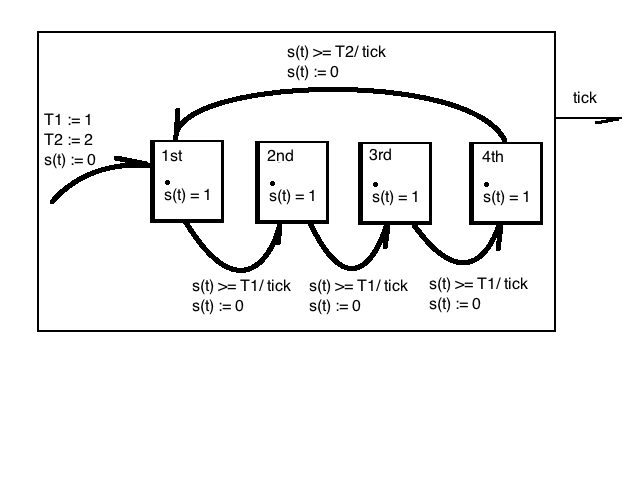
\includegraphics[scale=0.7]{hw7_1_actor_detail.png}
%% http://cremeronline.com/LaTeX/minimaltikz.pdf
\caption{Hybrid timed automata}
\label{fig:time_automata}
\end{figure}

The formal model is that of a hybrid automaton.
\begin{equation}
H = (Q, X, Init, f, Inv, E, G, R)
\end{equation}

The set of discrete variables.
\begin{equation}
Q & = \{1st, 2nd, 3rd, 4th\}
\end{equation}

The set of continuous variables.
$X = \mathbb{R}$
\begin{equation}
X = \{s(t)\}
\end{equation}

The set of initial conditions.
$Init \subseteq Q \times X$
\begin{equation}
Init = \{ ( 1st, s(t)} := 0 ) \}
\end{equation}

The vector field.
$f: Q \times X$
\begin{align}
f = \{ & ( 1st, \dot{s(t)}),  1 ) \\
    & ( 2nd, \dot{s(t)}), 1 ) \\
    & ( 3rd, \dot{s(t)}), 1 ) \\
    & ( 4th, \dot{s(t)}), 1 ) \}
\end{align}

The invariant set. (all empty)
$Q \mapsto 2^X$
\begin{align}
Inv = \{ & ( 1st, \emptyset ) \\
    & ( 2nd, \emptyset ) \\
    & ( 3rd, \emptyset ) \\
    & ( 4th, \emptyset ) \}
\end{align}

The collection of discrete transitions.
$E \subset Q \times Q$
\begin{align}
E = \{ & ( 1st, 2nd ) \\
    & ( 2nd, 3rd ) \\
    & ( 3rd, 4th ) \\
    & ( 4th, 1st ) \}
\end{align}

The guards on the transitions.
$G: E \mapsto 2^X$
\begin{align}
G = \{ & (( 1st, 2nd ), s(t) >= T_1 / tick ) \\
    & (( 2nd, 3rd ), s(t) >= T_1 / tick \\
    & (( 3rd, 4th ), s(t) >= T_1 / tick \\
    & (( 4th, 1st ), s(t) >= T_2 / tick \}
\end{align}

The reset relation on the transitions.
$R: E \times X \mapsto 2^X$
\begin{align}
R = \{ & (( 1st, 2nd , s(t)),  0 ) \\
    & (( 2nd, 3rd , s(t)), 0 \\
    & (( 3rd, 4th , s(t)), 0  \\
    & (( 4th, 1st , s(t)), 0  \}
\end{align}

\section{Automobile Features}

\subsection{Dome Light}
The dome light is turned on as soon as any door
is opened.
It stays on for 30 seconds after all doors are shut.
A sensor which can detect when a door's position,
$\{opened, closed\}$ is needed for each door.

\begin{figure}[h!]
\centering
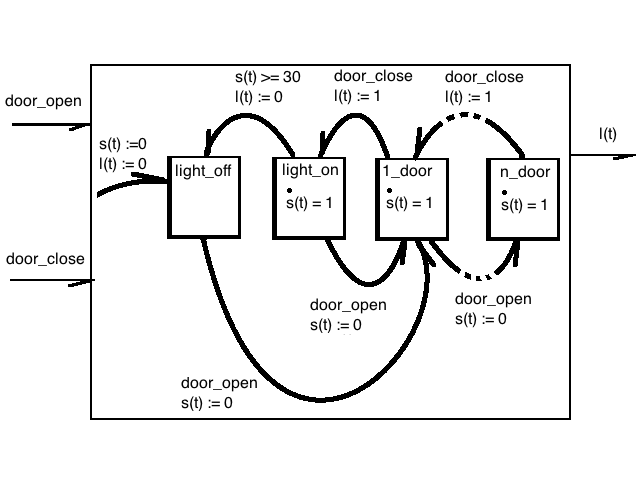
\includegraphics[scale=0.7]{hw7_4a_actor_dome.png}
\caption{A dome light}
\label{fig:dome_light}
\end{figure}


The formal model is that of a hybrid automaton.
\begin{equation}
H = (Q, X, Init, f, Inv, E, G, R)
\end{equation}

The set of discrete variables.
\begin{equation}
Q & = \{light_{off}, light_{on}, door_1, door_2, \ldots, door_n \}
\end{equation}

The set of continuous variables.
$X = \mathbb{R}$
\begin{equation}
X = \{ s(t), l(t) \}
\end{equation}

The set of initial conditions.
$Init \subseteq Q \times X$
\begin{equation}
Init = \{ ( light_{off}, l(t)} := 0 , s(t) := 0) \}
\end{equation}

The vector field.
$f: Q \times X$
\begin{align}
f = \{ & ( light_{off}, \dot{s(t)}), 1 ) \\
    & ( light_{on}, \dot{s(t)}), 1 ) \\
    & ( door_1, \dot{s(t)}), 1 ) \\
    & \ldots \\
    & ( door_n, \dot{s(t)}), 1 ) \}
\end{align}

The invariant set. (all empty)
$Q \mapsto 2^X$
\begin{align}
Inv = \{ & ( light_{off}, \emptyset ) \\
    & ( light_{on}, \emptyset ) \\
    & ( door_1, \emptyset ) \\
    & \ldots \\
    & ( door_n, \emptyset ) \}
\end{align}

The collection of discrete transitions.
$E \subset Q \times Q$
\begin{align}
E = \{ & ( light_{off}, door_1 ) \\
    & ( light_{on}, door_1 ) \\
    & ( door_1, door_2 ) \\
    & \ldots \\
    & ( door_{n-1}, door_n ) \\
    & ( door_n, door_{n-1} ) \\
    & \ldots \\
    & ( door_2, door_1 ) \\
    & ( door_1, light_{on} ) \\
    & ( light_{on}, light_{off} ) \}
\end{align}

The guards on the transitions.
$G: E \mapsto 2^X$
\begin{align}
G = \{ & ( light_{off}, door_1 ) \mapsto door_{open} \\
    & ( light_{on}, door_1 ) \mapsto door_{open} \\
    & ( door_1, door_2 ) \mapsto door_{open} \\
    & \ldots \\
    & ( door_{n-1}, door_n ) \mapsto door_{open} \\
    & ( door_n, door_{n-1} ) \mapsto door_{close} \\
    & \ldots \\
    & ( door_2, door_1 ) \mapsto door_{close} \\
    & ( door_1, light_{on} ) \mapsto door_{close} \\
    & ( light_{on}, light_{off} \mapsto s(t) \geq 30 ) \}
\end{align}

The reset relation on the transitions.
$R: E \times X \mapsto 2^X$
\begin{align}
R = \{ & ( light_{off}, door_1 ) \mapsto s(t) := 0 \\
    & ( light_{on}, door_1 ) \mapsto  s(t) := 0 \\
    & ( door_1, door_2 ) \mapsto  s(t) := 0 \\
    & \ldots \\
    & ( door_{n-1}, door_n ) \mapsto  s(t) := 0 \\
    & ( door_n, door_{n-1} ) \mapsto l(t) := 1 \\
    & \ldots \\
    & ( door_2, door_1 ) \mapsto l(t) := 1 \\
    & ( door_1, light_{on} ) \mapsto l(t) := 1 \\
    & ( light_{on}, light_{off} \mapsto l(t) := 0 ) \}
\end{align}

\subsection{Safety Belt Alarm}
Once the engine is runing,
a beeper is sounded and
a red light warning is indicated if thre are
passengers that have not buckled their seat belt.
The beeper stops sounding after 30 seconds, or
as soon as the seat belts are buckled,
whichever is sooner.
The warning light remains on so long as the
seatbelt on an occupied seat is not buckled.

The problem is made more tractable by
replacing the engine running condition with
the ignition on condition (for gasoline engines
this is a reasonable assumption).


Each seat has two sensors, one indicating that
the $seat \in \{occupied empty\}$
and one indicating that the
$seatbelt \in \{buckled unbuckled\}$.
Another sensor indicates
$ignition \in \{on off\}$
In the diagram only the driver and one passenger
seat witll be shown.
The formal model will be extended to $n$ seats.

Actuators $light_{warning} \in \{on off\}$
and $beeper_{warning} \in \{on off\}$ are present.

$warn$ \is an event generated when the $ignition$ is
turned $on$ and any $seat$ is $occupied$ or when
the $ignition$ is already $on$ and a $seat$ becomes
occupied.

\begin{figure}[h!]
\centering
\includegraphics[scale=0.3]{hw7_4b_formal_model.jpg}
\caption{The formal model elements}
\label{fig:4b_formal_model}
\end{figure}

The model consists of three types of connected agent models.

$noWarn$ is an event generated when a $seatbelt$ is $buckled$
a $seat$ becomes $empty$ or the $ignition$ is turned $off$.

\begin{figure}[h!]
\centering
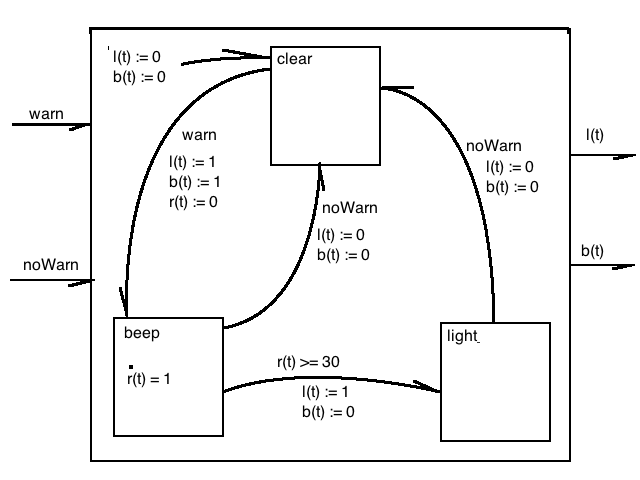
\includegraphics[scale=0.1]{hw7_4b_actor_total.jpg}
\caption{The final actor environment}
\label{fig:4b_actor_total_env}
\end{figure}

\begin{figure}[h!]
\centering
\includegraphics[scale=0.3]{hw7_4b_actor_total_detail.jpg}
\caption{The final actor detail}
\label{fig:4b_actor_total_detail}
\end{figure}

The $warn$ and $noWarn$ inputs to the total model are
produced by an aggregation agent with combines the
events for the individual $seats_i$.

\begin{figure}[h!]
\centering
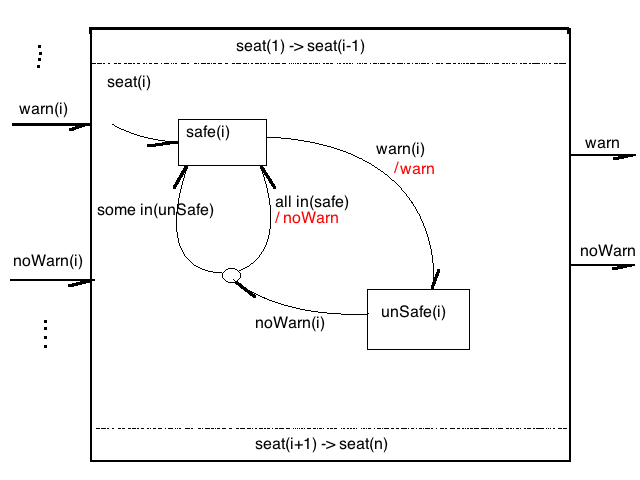
\includegraphics[scale=0.1]{hw7_4b_actor_aggr.jpg}
\caption{The aggregate actor environment}
\label{fig:4b_actor_aggr_env}
\end{figure}

\begin{figure}[h!]
\centering
\includegraphics[scale=0.3]{hw7_4b_actor_aggr_detail.jpg}
\caption{The aggregate actor detail}
\label{fig:4b_actor_aggr_detail}
\end{figure}

Feeding into the aggregator agent are $n$ seats.


\begin{figure}[h!]
\centering
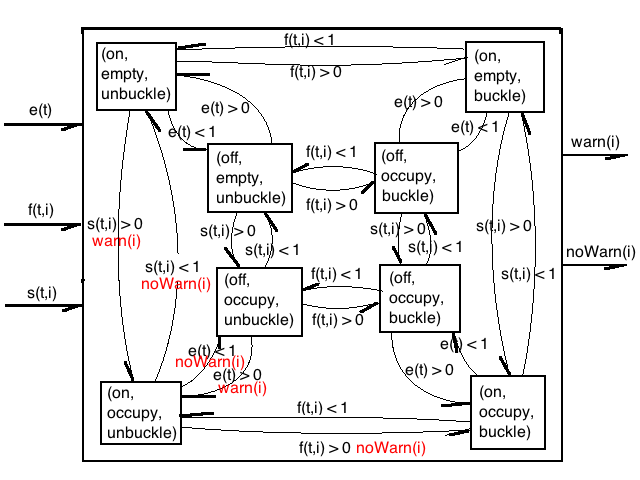
\includegraphics[scale=0.1]{hw7_4b_actor_seat.jpg}
\caption{A seat actor environment}
\label{fig:4b_actor_seat_env}
\end{figure}

\begin{figure}[h!]
\centering
\includegraphics[scale=0.3]{hw7_4b_actor_seat_detail.jpg}
\caption{A seat actor detail}
\label{fig:4b_actor_seat_detail}
\end{figure}

\end{document}
